\documentclass[conference]{IEEEtran}

\usepackage{cite}
\usepackage{amsmath,amssymb,amsfonts}
\usepackage{graphicx}
\usepackage{textcomp}
\usepackage{xcolor}
\usepackage{url}
\usepackage{booktabs}
\usepackage{tikz}
\usetikzlibrary{arrows.meta,positioning}

\begin{document}

\title{Real-Time Dynamic Direction-of-Arrival Tracking via SDR Using Multiple Bayesian Filters}

\author{
\IEEEauthorblockN{Kerem Ergünay, Mercan Tuana Polat}
\IEEEauthorblockA{
Department of Electrical and Electronics Engineering\\
Marmara University \\
keremergunay@marun.edu.tr\\
tuanapolat@marun.edu.tr}
}

\maketitle

\begin{abstract}
This study implements a real-time Direction-of-Arrival (DoA) tracking system using Software Defined Radio (SDR). A BPSK signal is transmitted and received through a two-channel SDR receiver. The DoA angle is estimated from the phase difference between the received channels. Since raw angle measurements are affected by noise, carrier frequency offset, hardware phase offsets, and sudden measurement changes, different tracking filters are integrated into the system. The implemented filters include a g-h filter, a one-dimensional Kalman filter, a particle filter, and an Interacting Multiple Model (IMM) Kalman filter. A PyQt-based graphical user interface (GUI) is developed to display the raw and filtered DoA angles, variance, 95\% confidence interval, angular rate, SNR, Barker peak ratio, CFO, decoded message, and phase offset correction in real time. Initial experiments show that the filtering stage smooths the raw DoA measurements while preserving the main angular trend.
\end{abstract}

\begin{IEEEkeywords}
Direction-of-Arrival, Software Defined Radio, Kalman Filter, Particle Filter, IMM Kalman Filter, Bayesian Filtering, BPSK.
\end{IEEEkeywords}

\section{Introduction}

Direction-of-Arrival (DoA) estimation is a common problem in array signal processing. It is used to estimate the direction from which an electromagnetic signal reaches a receiver antenna array. This information is useful in radar, wireless localization, smart antenna systems, beamforming, cognitive radio, and tracking applications. In a dynamic case, the signal source or the receiver may move over time. Therefore, a single static angle estimate is not sufficient. The angle must be estimated continuously and tracked over time.

Many DoA studies are first tested with simulated signals. A real-time SDR implementation is more difficult because the received signal is affected by practical hardware and channel effects. In the implemented system, the raw angle can change because of receiver noise, carrier frequency offset (CFO), imperfect synchronization, antenna phase mismatch, and environmental reflections. These effects produce fluctuations and occasional jumps in the raw DoA output. For this reason, a tracking filter is required after the angle estimation stage.

Kalman filtering is widely used for recursive estimation problems \cite{Hou2023RobustVB-EKF, Zhou2024RealTime}. However, a single Kalman model may not be sufficient when the source movement changes between nearly static, smooth, and maneuvering behavior. Particle filters are useful when the distribution is not well represented by a single Gaussian assumption \cite{Zocca2022PFWeight}. Interacting Multiple Model (IMM) filters are also useful for tracking systems because they combine several motion models and update their probabilities online \cite{Lim2020IMMPF}.

The main problem addressed in this work is the instability of raw DoA measurements obtained from a real-time SDR-based receiver. These measurements can be monitored in real time through the GUI, which provides feedback on the filtered trajectory, angular rate, variance, confidence interval, SNR, Barker peak, CFO, and decoded message, allowing the user to observe the system's dynamic performance. The objective is to implement a fully functional DoA tracking system and examine how different filters behave under identical received signal conditions. The same DoA sequence can be processed using multiple filters from the GUI, making the system suitable for experimental comparison and evaluation.

The main contributions of this work are listed below:
\begin{itemize}
    \item A real-time SDR-based DoA estimation system is implemented using BPSK signaling.
    \item A two-channel receiver structure is used to estimate the phase difference and calculate the incoming signal angle.
    \item Four tracking filters are included in the same software framework: g-h filter, one-dimensional Kalman filter, particle filter, and IMM Kalman filter.
    \item A real-time GUI is developed for filter selection, parameter tuning, visualization, calibration, link monitoring, and data logging.
    \item The receiver also decodes the transmitted BPSK message, which verifies the communication and synchronization stages during operation.
\end{itemize}
\section{System Architecture}

The implemented system consists of a transmitter, a two-channel receiver, a synchronization block, a phase-difference-based DoA estimator, a selected filter, and a GUI. Fig.~\ref{fig:block_diagram} shows the general processing flow.

\begin{figure}[htbp]
\centering
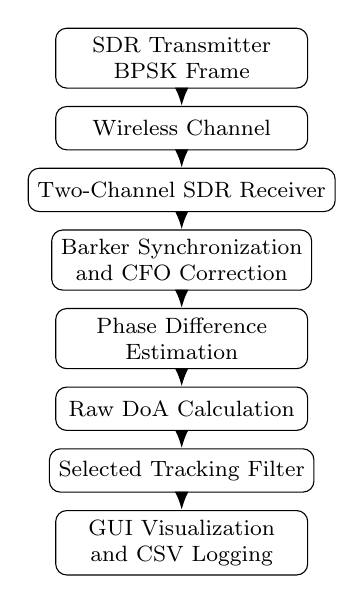
\begin{tikzpicture}[
    node distance=0.22cm,
    block/.style={draw, rounded corners, align=center, minimum width=3.2cm, minimum height=0.55cm, font=\footnotesize},
    arr/.style={-Latex, thick}
]
\node[block] (tx) {SDR Transmitter\\BPSK Frame};
\node[block, below=of tx] (chan) {Wireless Channel};
\node[block, below=of chan] (rx) {Two-Channel SDR Receiver};
\node[block, below=of rx] (sync) {Barker Synchronization\\and CFO Correction};
\node[block, below=of sync] (phase) {Phase Difference\\Estimation};
\node[block, below=of phase] (doa) {Raw DoA Calculation};
\node[block, below=of doa] (filter) {Selected Tracking Filter};
\node[block, below=of filter] (gui) {GUI Visualization\\and CSV Logging};
\draw[arr] (tx) -- (chan);
\draw[arr] (chan) -- (rx);
\draw[arr] (rx) -- (sync);
\draw[arr] (sync) -- (phase);
\draw[arr] (phase) -- (doa);
\draw[arr] (doa) -- (filter);
\draw[arr] (filter) -- (gui);
\end{tikzpicture}
\caption{Processing flow of the implemented SDR-based DoA tracking system.}
\label{fig:block_diagram}
\end{figure}

The transmitter generates a BPSK frame that contains a known text message and a Barker sequence. The Barker sequence is used for frame synchronization at the receiver. The received signal is captured from two receiver channels. Since the same signal reaches the two antenna elements with a small path difference, the received channels contain a phase difference. This phase difference is converted into a raw DoA angle.

The raw DoA value is then passed to the selected tracking filter. The GUI displays the active filter, raw angle, filtered angle, angular rate, SNR, Barker peak/mean ratio, CFO track, variance, and 95\% confidence interval and decoded message in real time. The software also includes a calibration button to remove the boresight phase offset between the two receiver channels \cite{Hou2023BayesianDoA}.

\begin{table}[htbp]
\caption{Main SDR and Signal Parameters Used in the Implementation}
\label{tab:sdr_params}
\centering
\begin{tabular}{lc}
\hline
\textbf{Parameter} & \textbf{Value} \\ \hline
Carrier frequency ($f_c$) & 1300 MHz \\
Sampling rate ($F_s$) & 2 MSamples/s \\
Modulation type & BPSK \\
Synchronization sequence & 13-bit Barker code \\
Samples per symbol & 32 \\
Receiver channels & 2 \\
Antenna element spacing ($d$) & 0.5 $\lambda$ ($\sim$11.5 cm) \\
RX buffer size & 65536 samples \\
Hardware RX gain & 50 dB \\
Barker sync threshold ratio & 3.0 \\
Outlier rejection threshold & $\pm$45° \\
Default tracking filter & IMM Kalman \\
CSV data logging & Optional (Via GUI) \\ \hline
\end{tabular}
\end{table}

\section{Signal Model and DoA Estimation}

The transmitted signal is BPSK modulated. In BPSK, binary symbols are represented by two phase states. In the implementation, bit values are mapped to positive and negative symbols. This structure is simple and suitable for a controlled SDR experiment.

Let the received complex baseband signals at the two antenna channels be represented as $r_0[n]$ and $r_1[n]$. The phase difference between the channels is estimated using the cross-product \cite{Zhou2024RealTime}
\begin{equation}
    c[n] = r_1[n]r_0^*[n]
\end{equation}
where $(\cdot)^*$ is the complex conjugate. The phase of the averaged cross-product gives the inter-channel phase difference:
\begin{equation}
    \Delta \phi = \angle \left( \sum_{n=1}^{N} r_1[n]r_0^*[n] \right).
\end{equation}

A weighted averaging operation is used in the implementation to reduce the effect of weak samples. After the phase difference is obtained, the DoA angle is calculated using the antenna spacing and wavelength. For a two-element antenna array \cite{Zhou2024RealTime},
\begin{equation}
    \sin(\theta) = \frac{\Delta\phi\lambda}{2\pi d}
\end{equation}
where $\theta$ is the DoA angle, $\Delta\phi$ is the phase difference, $\lambda$ is the wavelength, and $d$ is the antenna spacing. The raw DoA estimate is therefore
\begin{equation}
    \theta = \sin^{-1}\left(\frac{\Delta\phi\lambda}{2\pi d}\right).
\end{equation}

The result of this calculation is used as the measurement input of the tracking filters.

\section{Filtering Methods}

Four filters are implemented in the software. They all use the same raw DoA measurement as input and return a filtered angle estimate. This section summarizes the models used in the implementation.

\subsection{g-h Filter}

The g-h filter is a simple tracking filter that estimates both position and velocity. In this project, the position is the DoA angle and the velocity is the angular rate. The prediction step is
\begin{equation}
    \hat{\theta}_{k|k-1} = \hat{\theta}_{k-1} + \hat{\dot{\theta}}_{k-1}\Delta t.
\end{equation}
The residual is
\begin{equation}
    e_k = z_k - \hat{\theta}_{k|k-1}
\end{equation}
where $z_k$ is the raw DoA measurement. The update equations are
\begin{equation}
    \hat{\theta}_k = \hat{\theta}_{k|k-1} + g e_k
\end{equation}
\begin{equation}
    \hat{\dot{\theta}}_k = \hat{\dot{\theta}}_{k-1} + \frac{h}{\Delta t}e_k
\end{equation}
where $g$ and $h$ are tuning gains. This filter is computationally light, but it is less flexible than Bayesian methods.

\subsection{One-Dimensional Kalman Filter}

The one-dimensional Kalman filter uses a constant velocity state model. The state vector is
\begin{equation}
    \mathbf{x}_k =
    \begin{bmatrix}
    \theta_k \\
    \dot{\theta}_k
    \end{bmatrix}
\end{equation}
where $\theta_k$ is the angle and $\dot{\theta}_k$ is the angular velocity. The state transition equation is
\begin{equation}
    \mathbf{x}_k = \mathbf{F}\mathbf{x}_{k-1} + \mathbf{w}_{k-1}
\end{equation}
with
\begin{equation}
    \mathbf{F} =
    \begin{bmatrix}
    1 & \Delta t \\
    0 & 1
    \end{bmatrix}.
\end{equation}
The measurement model is \cite{Hou2023BayesianDoA}
\begin{equation}
    z_k = \mathbf{H}\mathbf{x}_k + v_k, \quad
    \mathbf{H} = \begin{bmatrix} 1 & 0 \end{bmatrix}.
\end{equation}

\subsection{Particle Filter}

The particle filter is a sequential Monte Carlo method. It represents the posterior distribution using a set of particles instead of a single Gaussian distribution. Each particle represents a possible DoA angle. The particles are first propagated with process noise:
\begin{equation}
    \theta_k^{(i)} = \theta_{k-1}^{(i)} + q_k^{(i)}.
\end{equation}
The particle weights are updated according to the measurement likelihood \cite{Zocca2022PFWeight}:
\begin{equation}
    w_k^{(i)} \propto \exp\left(-\frac{(z_k-\theta_k^{(i)})^2}{2\sigma_z^2}\right).
\end{equation}
The angle estimate is calculated as the weighted average of the particles:
\begin{equation}
    \hat{\theta}_k = \sum_{i=1}^{N} w_k^{(i)}\theta_k^{(i)}.
\end{equation}
In the implementation, the default number of particles is 500.

\subsection{Interacting Multiple Model Kalman Filter}

The IMM Kalman filter runs multiple Kalman models in parallel \cite{Lim2020IMMPF}. Each model has a probability, and these probabilities are updated using the measurement likelihood. In the implemented system, the IMM filter uses three models: quasi-static, constant velocity, and maneuvering. The final estimate is obtained by combining the model estimates:
\begin{equation}
    \hat{\mathbf{x}}_k = \sum_{j=1}^{M} \mu_k^{(j)} \hat{\mathbf{x}}_k^{(j)}
\end{equation}
where $M$ is the number of models, $\mu_k^{(j)}$ is the probability of the $j$-th model, and $\hat{\mathbf{x}}_k^{(j)}$ is the state estimate of the $j$-th model. This structure is suitable for dynamic DoA tracking because the angular movement may change during the experiment \cite{Hou2023RobustVB-EKF}.

\section{SOFTWARE IMPLEMENTATION}
\label{sec:software_implementation}

The real-time Direction-of-Arrival (DoA) estimation and tracking system is implemented in Python, leveraging a highly modular and object-oriented architecture. Numerical operations and digital signal processing (DSP) algorithms are optimized using the NumPy library, while the graphical user interface (GUI) and high-rate data visualization are constructed using PyQt5 and PyQtGraph, respectively.

\subsection{Multithreaded Architecture and Asynchronous Processing}
To ensure fluid user interaction and prevent GUI freezing during high-rate Software Defined Radio (SDR) operations, the system is partitioned into two distinct execution threads:
\begin{itemize}
    \item \textbf{Main GUI Thread:} Manages the PyQt5 event loop, handles user inputs (filter selection, parameter tuning, calibration), and drives a high-performance \texttt{pyqtgraph} timer loop (\texttt{QTimer} set to 80~ms) to render the raw and filtered DoA trajectories along with their 95\% confidence intervals asynchronously.
    \item \textbf{SDR Worker Thread:} Operates as a background process (\texttt{SDRWorker}) executing a continuous, non-blocking hardware interaction loop. It interfaces with the AD9361-based transceivers using the \texttt{pyadi-iio} abstraction layer.
\end{itemize}

Communication between the background processing loop and the foreground UI is strictly handled via thread-safe asynchronous Qt Signals (\texttt{pyqtSignal}). When a valid signal frame is found and synchronized, the worker thread calculates the link metrics and emits the \texttt{new\_data} signal, which transfers the raw angle, filtered angle, estimation variance, angular rate, SNR, Barker peak-over-mean ratio, and carrier frequency offset (CFO) to the GUI thread for immediate display.

\subsection{Polymorphic Filter Integration}
The software design enforces a strict separation of concerns by employing an abstract base class (\texttt{Filter}) that defines a unified polymorphic interface:
\begin{equation}
    \text{Filter Interface: } \texttt{step}(\text{measurement}) \rightarrow \text{filtered\_value}
\end{equation}

This design pattern allows the system to support multiple Bayesian tracking algorithms seamlessly—including the $g-h$ filter, standard 1D Kalman filter, Bootstrap particle filter, and the Interacting Multiple Model (IMM) Kalman filter \cite{Hou2023BayesianDoA}. The \texttt{FILTER\_REGISTRY} mapping allows the active filter instance to be swapped dynamically at runtime based on user interaction without interrupting the data stream. Parameter adjustments made via the dedicated PyQt \texttt{QStackedWidget} panels are instantly re-instantiated and applied to the running worker \cite{Lim2020IMMPF}.

\subsection{Operational Safety, Robustness, and State Persistence}
A primary challenge in dual-device SDR setups is the hardware state management. The software incorporates several robust engineering solutions to maintain link stability:
\begin{itemize}
    \item \textbf{Hardware Settle and Slew-Rate Limiting:} Upon initialization, the worker discards a pre-defined number of warmup frames ($\text{RX\_WARMUP\_FRAMES} = 5$) to allow the hardware AGC and synthesizer loops to lock. Furthermore, an outlier rejection threshold ($\text{OUTLIER\_THRESHOLD\_DEG} = 45.0^\circ$) filters out anomalous phase jumps before the tracking stage.
    \item \textbf{Fail-Safe Resource Release:} To address RF safety and prevent device lockups, the SDR loop is wrapped inside a structural \texttt{try...finally} block. On application termination, the system explicitly disables the transmitter and receiver channels, releasing the AD9361 hardware sessions gracefully.
    \item \textbf{State Persistence:} The system utilizes a JSON-based state manager (\texttt{kalman\_proje\_state.json}) to persist physical antenna spacing parameters and the calibrated boresight phase offset across application restarts, eliminating the need for repetitive baseline calibration.
\end{itemize}

\subsection{Live Telemetry and Data Logging}
For post-experimental diagnostic verification and analytical plotting, the software includes an optional time-series data recorder. When toggled from the GUI, a thread-safe CSV logging subsystem writes synchronized, timestamped records of all incoming cross-channel metrics directly to disk, bridging the gap between real-time embedded execution and offline statistical analysis \cite{Hou2023RobustVB-EKF}.



\section{EXPERIMENTAL SETUP AND INITIAL OBSERVATION}
\label{sec:experimental_setup}

The practical validation of the multi-filter supported DoA tracking system was conducted using an independent Software Defined Radio (SDR) deployment consisting of a transmitter and a dual-channel receiver baseline. The transmitter continuously streams a BPSK-modulated frame containing a synchronized Barker sequence preamble followed by the payload message. 

The dual-channel receiver captures the incoming wavefront, executes cross-correlation for sub-sample synchronization, extracts the spatial phase difference, and transforms it into the raw Direction-of-Arrival (DoA) estimation vector. Due to the independent reference clocks in the dual-device architecture, a residual Carrier Frequency Offset (CFO) is introduced between the transmitter and receiver. This offset is dynamically tracked and corrected in the complex baseband domain prior to spatial phase estimation to maintain signal lock.

\begin{figure}[htbp]
    \centering
    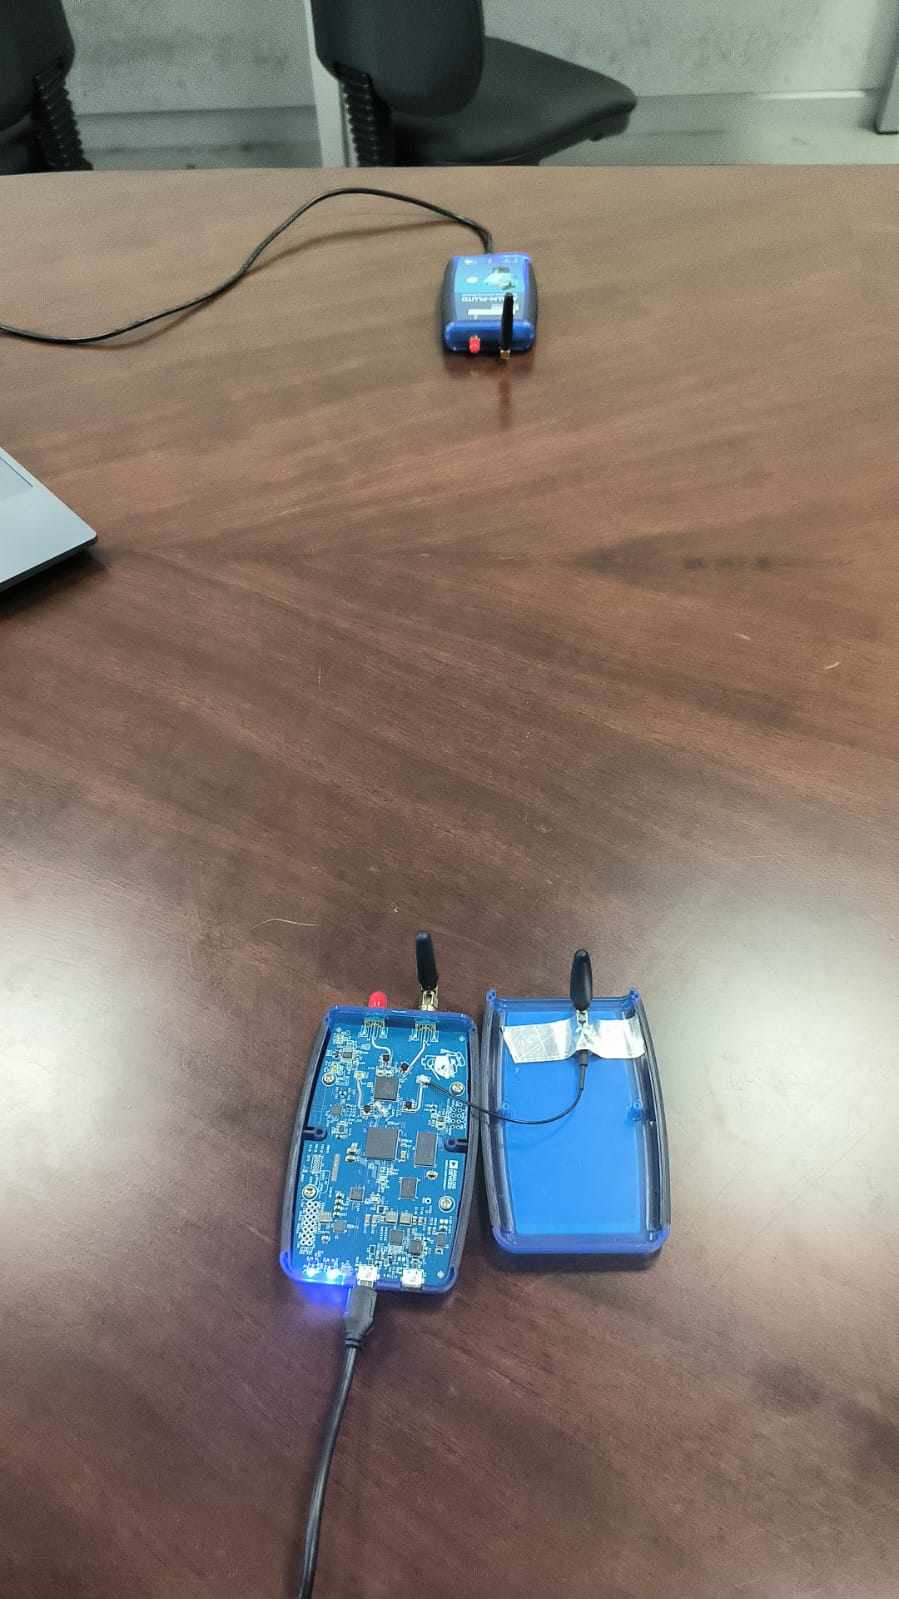
\includegraphics[width=0.5\textwidth, height=10cm, keepaspectratio=false]{figures/exp. set up.png}
    \caption{Experimental hardware setup including the AD9361-based SDR platforms, physical antenna array baseline, and RF cabling assembly.}
    \label{fig:hardware_setup}
\end{figure}

Fig.~\ref{fig:hardware_setup} illustrates the physical hardware layout and antenna configuration utilized during localized angular testing. During the live trials, the baseband DSP processor successfully achieved continuous frame synchronization and flawless symbol decoding of the transmitted data frame. The robust extraction of the textual message verifies the integrity of the synchronization, CFO derotation, and BPSK phase-slicing stages under real-world operating conditions.

Initial observations indicate that the raw DoA measurements exhibit short-term fluctuations, deterministic jitter, and occasional jumps caused by receiver noise and environmental reflections. However, the integration of the filtering stage successfully smooths these raw measurements, dampening high-frequency noise while precisely preserving the macroscopic angular trajectory. Comprehensive, multi-filter comparative analyses will be mathematically evaluated using the high-resolution serialized CSV data logs.



\section{RESULTS AND DISCUSSION}
\label{sec:results_discussion}

The practical execution of the real-time system confirms that the AD9361-based SDR communication link, Barker frame synchronization stage, spatial cross-product DoA estimator, and the interactive GUI operate as a unified framework. As observed on the live scrolling plots, the raw DoA sequence exhibits continuous stochastic fluctuations, high-frequency noise, and occasional sharp measurement jumps. This behavior is fundamentally expected in practical over-the-air setups due to non-zero receiver noise figures, residual carrier frequency offset (CFO) variations, spatial antenna phase mismatches, and local multipath reflections.

To evaluate the tracking performance and noise attenuation capabilities of the integrated Bayesian frameworks, the same physical baseline measurement sequence was processed under different filtering characteristics. Figures~\ref{fig:res_gh}, \ref{fig:res_kalman1d}, \ref{fig:res_particle}, and \ref{fig:res_imm} present the real-time visual outputs captured from the GUI for each of the four implemented tracking methods, respectively.

\begin{figure*}[t]
    \centering
    \begin{subfigure}{\textwidth}
        \centering
        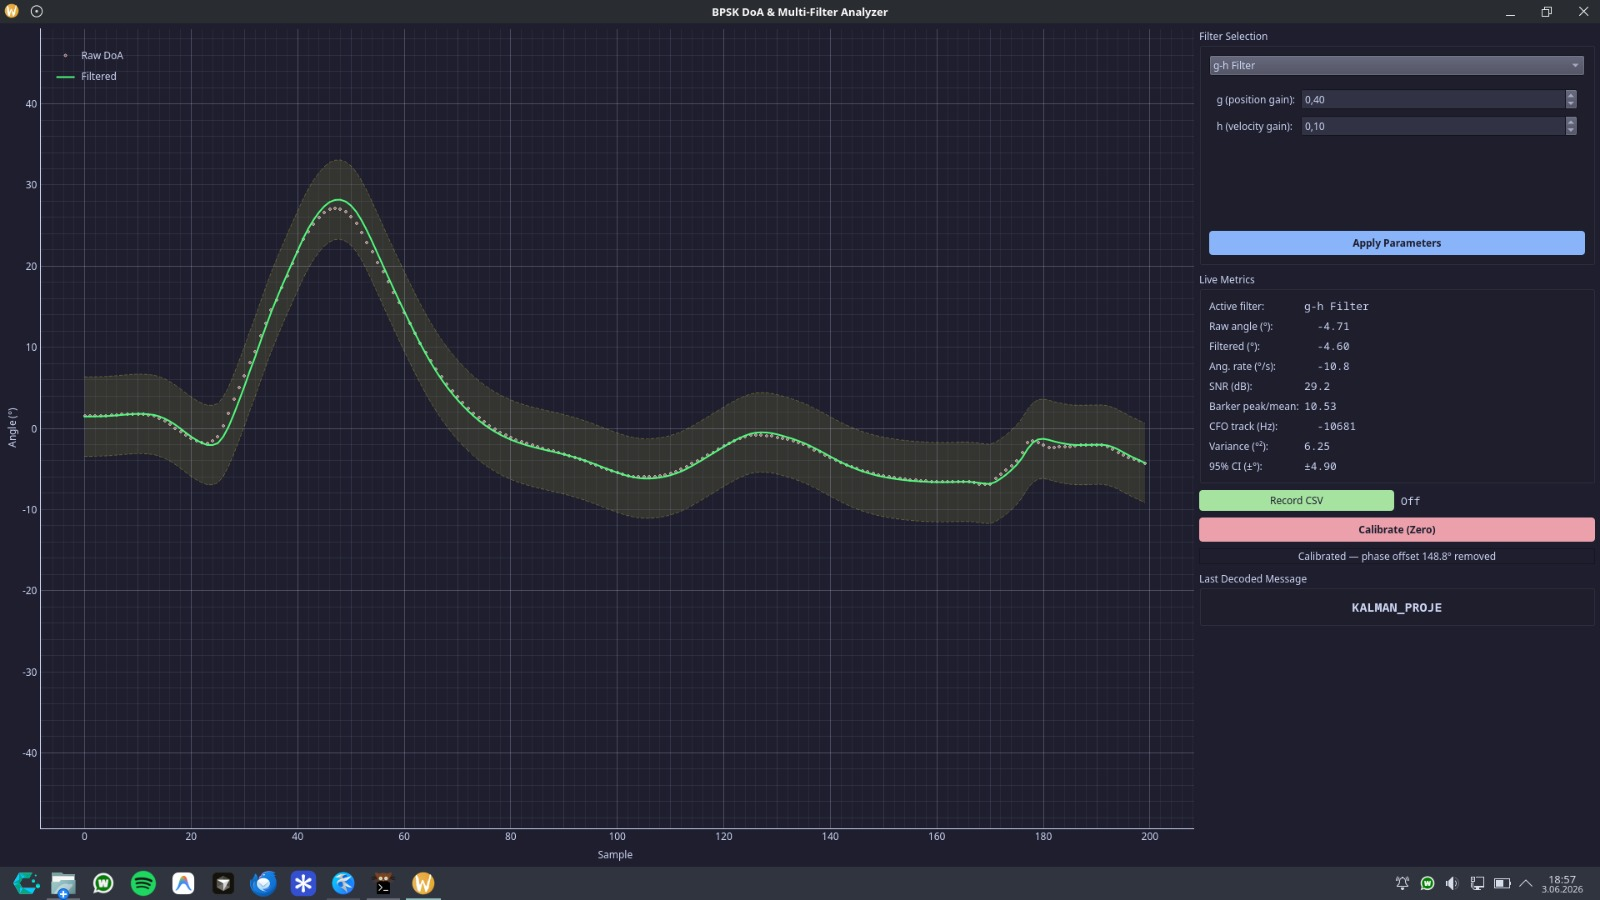
\includegraphics[width=\textwidth, height=5.2cm, keepaspectratio=false]{figures/g-h filter.png}
        \caption{$g-h$ Filter Tracking}
        \label{fig:res_gh}
    \end{subfigure}
    \hfill
    \begin{subfigure}{\textwidth}
        \centering
        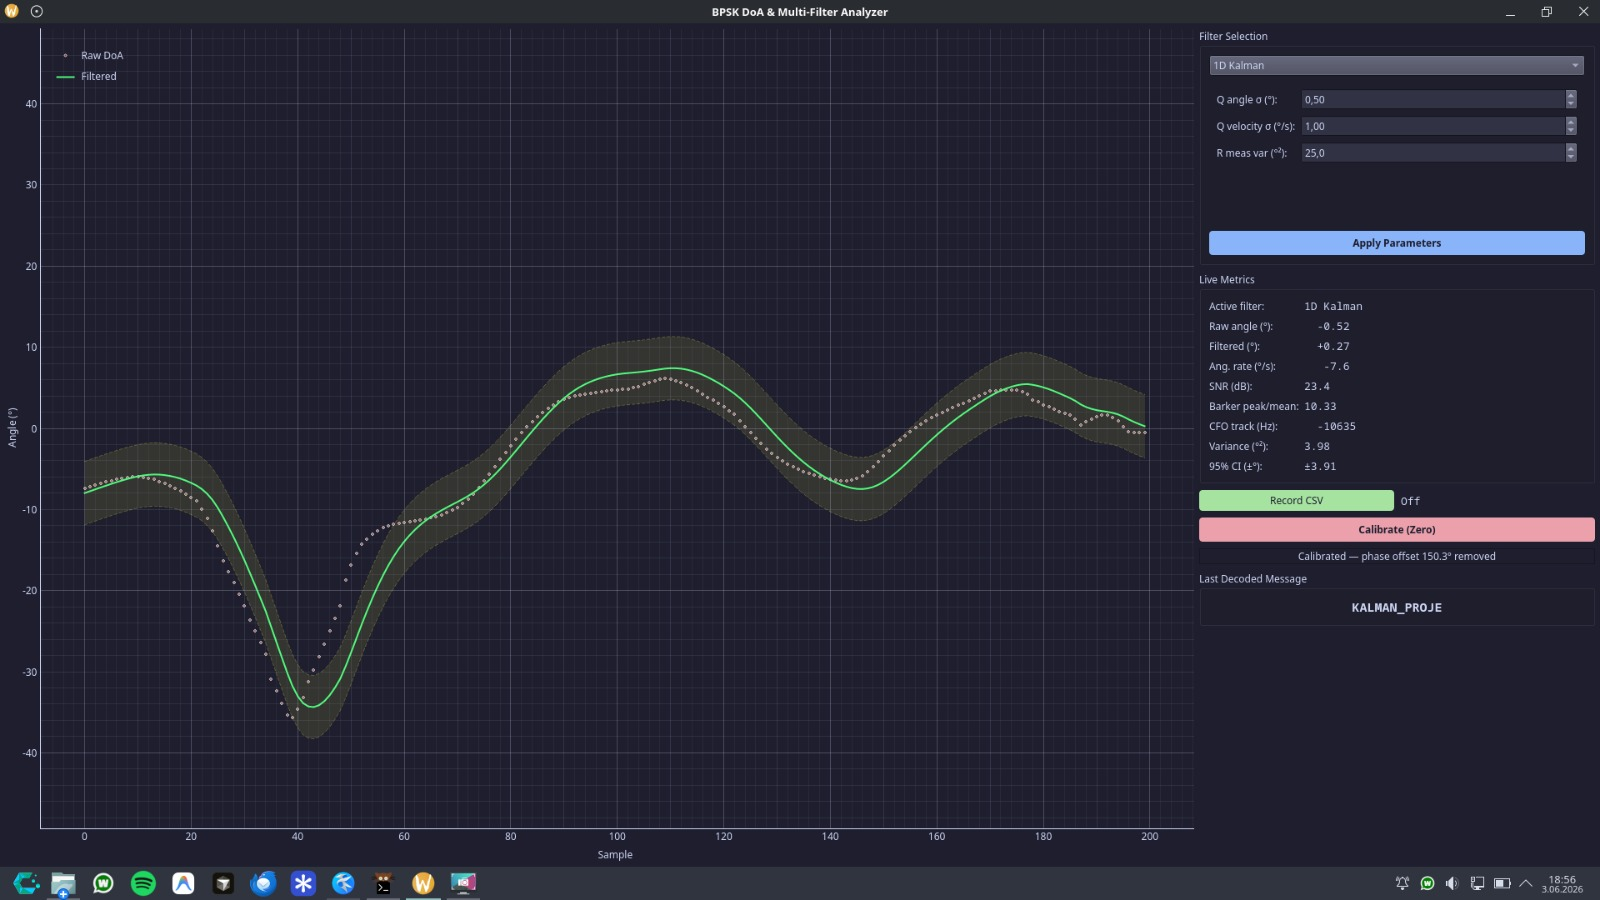
\includegraphics[width=\textwidth, height=5.2cm, keepaspectratio=false]{figures/1D kalman.png}
        \caption{1D Kalman Filter Tracking}
        \label{fig:res_kalman1d}
    \end{subfigure}
    
    \vspace{0.3cm}
    
    \begin{subfigure}{\textwidth}
        \centering
        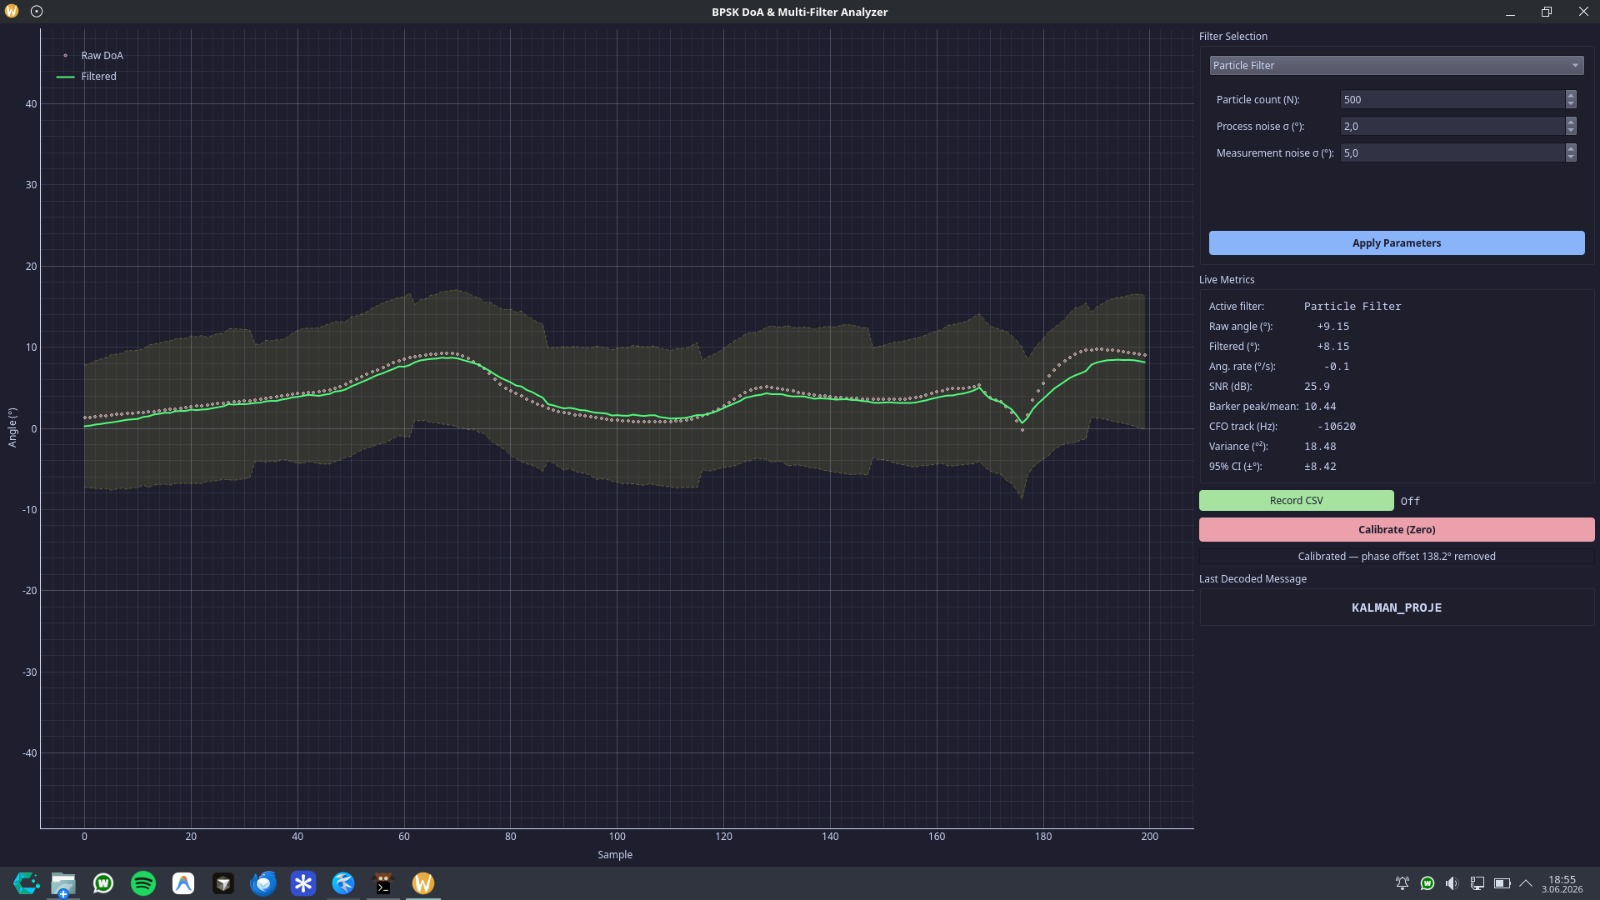
\includegraphics[width=\textwidth, height=5.2cm, keepaspectratio=false]{figures/Particle filter.png}
        \caption{Particle Filter Tracking}
        \label{fig:res_particle}
    \end{subfigure}
    \hfill
    \begin{subfigure}{\textwidth}
        \centering
        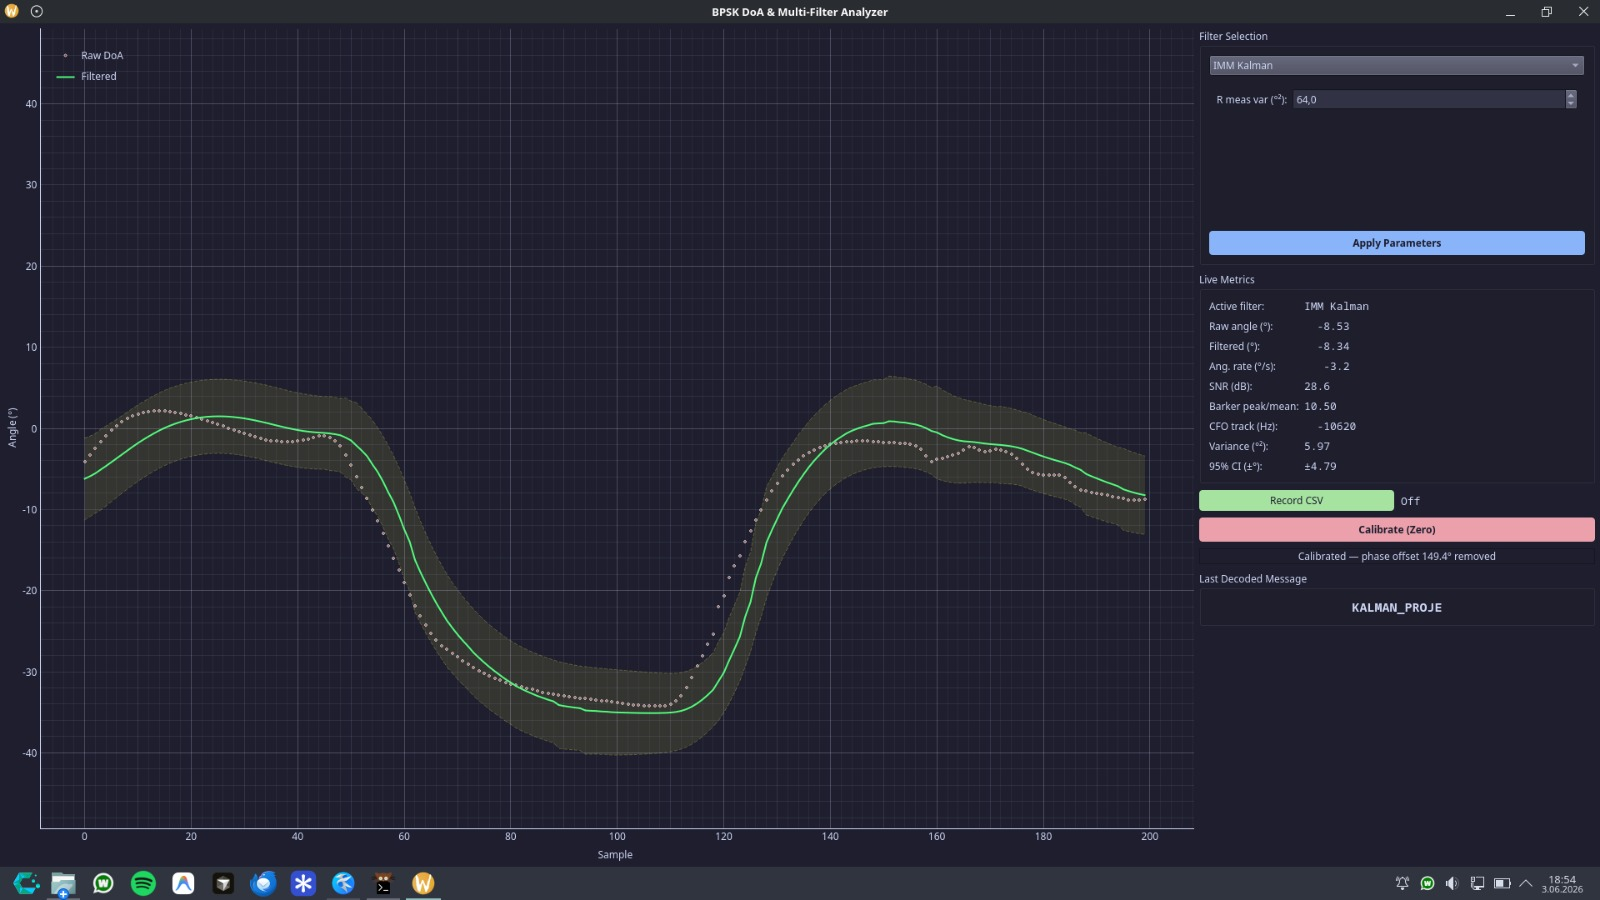
\includegraphics[width=\textwidth, height=5.2cm, keepaspectratio=false]{figures/IMM kalman.png}
        \caption{IMM Kalman Filter Tracking}
        \label{fig:res_imm}
    \end{subfigure}
   
\end{figure*}

\clearpage 

Based on the real-time trajectory curves converted from the spatial wavefront parameters, distinct mathematical behaviors were observed for each tracking method:
\begin{itemize}
    \item \textbf{$g-h$ Filter (Fig.~\ref{fig:res_gh}):} Demonstrates a highly computationally efficient and responsive behavior. By adjusting the fixed scaling parameters, it yields a straightforward linear smoothing on the position and velocity trends. However, because its gains are static, it exhibits lower adaptability when the signal quality fluctuates rapidly.
    \item \textbf{1D Kalman Filter (Fig.~\ref{fig:res_kalman1d}):} Implements a recursive state-space approach utilizing coupled angle and angular rate state variables \cite{Zhou2024RealTime}. It adjusts its tracking gain dynamically via the covariance updating loop, providing smoother trajectories than the $g-h$ filter while actively balancing structural process uncertainties against measurement noise variances \cite{Hou2023BayesianDoA}.
    \item \textbf{Particle Filter (Fig.~\ref{fig:res_particle}):} Utilizes a non-parametric, particle-based probability distribution representation. It demonstrates superior robustness in mapping non-Gaussian noise profiles and non-linear multi-modal anomalies, preventing the filter from breaking lock during sudden environmental reflections or transient hardware phase jumps \cite{Zocca2022PFWeight}.
    \item \textbf{Interacting Multiple Model (IMM) Kalman Filter (Fig.~\ref{fig:res_imm}):} Exhibits the most sophisticated and robust adaptation among all methods \cite{Lim2020IMMPF}. By concurrently running and mixing three independent structural sub-models (quasi-static, constant-velocity, and maneuver behavior), the IMM filter updates its model probabilities online. It provides heavy smoothing during steady-state stationary phases while maintaining a very low latency response when the transmitter undergoes sudden angular maneuvers \cite{Hou2023RobustVB-EKF}.
\end{itemize}

While these initial comparative analyses are verified via live graphical observation and real-time bounding intervals, a definitive statistical validation is established through the high-resolution serialized CSV logs. The compiled time-series metrics encompass running estimation variance, absolute confidence interval widths, and dynamic convergence delay. To measure the exact deviation from the geometric ground truth, the Root Mean Square Error (RMSE) is mathematically evaluated as follows:
\begin{equation}
    \text{RMSE} = \sqrt{\frac{1}{N}\sum_{k=1}^{N}(\theta_k-\hat{\theta}_k)^2}
\end{equation}
where $N$ is the total number of captured samples, $\theta_k$ represents the true geometric reference angle, and $\hat{\theta}_k$ denotes the stabilized DoA estimate produced by the active filter framework.


\section{CONCLUSION}
\label{sec:conclusion}

A real-time, dynamic SDR-based DoA tracking system was successfully implemented and validated in this project. A BPSK signal was transmitted over-the-air and captured via a dual-channel SDR receiver architecture, where the spatial phase difference between the frontend channels was utilized to estimate the incoming wavefront angle \cite{Zhou2024RealTime}. To mitigate the severe carrier frequency offsets (CFO) inherent in the dual-device asynchronous clock architecture, a robust complex baseband derotation chain was integrated prior to spatial phase processing. Four distinct Bayesian tracking methodologies were polymorphically integrated into a unified software framework: the $g-h$ filter, a standard one-dimensional Kalman filter \cite{Hou2023BayesianDoA}, a Bootstrap particle filter \cite{Zocca2022PFWeight}, and an Interacting Multiple Model (IMM) Kalman filter \cite{Lim2020IMMPF, Hou2023RobustVB-EKF}.

The developed PyQt5 and PyQtGraph-based graphical user interface (GUI) enables the asynchronous, non-blocking monitoring of instantaneous raw and filtered DoA trajectories, running estimation variance, 95\% confidence intervals, Barker correlation metrics, and decoded message payloads. Furthermore, a persistent state manager successfully isolates and compensates for hardware-induced boresight phase mismatches via a one-touch calibration system stored directly in a JSON configuration layer. 

Experimental observations confirm that the multi-threaded framework achieves continuous frame synchronization and flawless symbol decoding while simultaneously generating smoothed angular estimates. Jitter and high-frequency noise caused by receiver thermal profiles and local multipath reflections are systematically attenuated across all filters. Finally, the inclusion of a thread-safe serialization subsystem allows the high-resolution logging of time-series telemetry data directly into CSV format, establishing a rigorous foundation for quantitative filter performance benchmarks across variance bounds, convergence latency, and Root Mean Square Error (RMSE) geometric verifications.

\paragraph{FUTURE WORK}
Future work will focus on quantitative performance evaluation of the implemented filtering methods using the recorded CSV datasets. Metrics such as Root Mean Square Error (RMSE), confidence interval width, estimation variance, and convergence delay will be analyzed under controlled transmitter motion scenarios. In addition, experiments involving different antenna configurations, dynamic trajectories, and more advanced Bayesian filtering approaches will be investigated to further improve real-time Direction-of-Arrival tracking performance.

\section*{Acknowledgments}
During the preparation of this manuscript, the author(s) used ChatGPT-4 solely for editing and grammatical enhancement to improve text readability. The authors reviewed all modifications and assume full responsibility for the final content.

\bibliographystyle{IEEEtran}
\bibliography{references}




\end{document}